\documentclass{standalone}
\usepackage{fontspec}
\setsansfont{DejaVuSans.ttf}[Path=./,Kerning=Off,Ligatures={TeXOff,NoCommon}]
\usepackage{tikz}
\begin{document}
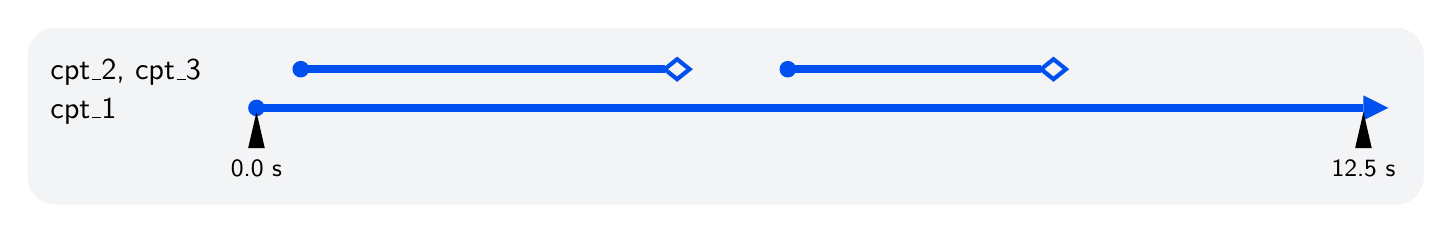
\begin{tikzpicture}[x=1pt,y=1pt,miter limit=4,font=\sffamily]
\definecolor{ts000000}{HTML}{000000}
\definecolor{ts0050EF}{HTML}{0050EF}
\definecolor{tsF3F4F6}{HTML}{F3F4F6}
\begin{scope}[shift={(16,16)}]
\path[rounded corners=10pt,fill=tsF3F4F6] (0,0) rectangle (504.4712,63.9766);
\path[draw=ts0050EF,line width=3pt] (82.6768,34.9766) -- (482.6768,34.9766);
\path[fill=ts0050EF] (82.6768,34.9766) circle[radius=3];
\path[fill=ts0050EF] (491.6768,34.9766) -- (482.6768,39.4766) -- (482.6768,30.4766) -- cycle;
\path[draw=ts0050EF,line width=3pt] (98.6768,48.9766) -- (230.1768,48.9766);
\path[fill=ts0050EF] (98.6768,48.9766) circle[radius=3];
\path[draw=ts0050EF,line width=1.5pt] (230.1768,48.9766) -- (234.6768,52.5766) -- (239.1768,48.9766) -- (234.6768,45.3766) -- cycle;
\path[draw=ts0050EF,line width=3pt] (274.6768,48.9766) -- (366.1768,48.9766);
\path[fill=ts0050EF] (274.6768,48.9766) circle[radius=3];
\path[draw=ts0050EF,line width=1.5pt] (366.1768,48.9766) -- (370.6768,52.5766) -- (375.1768,48.9766) -- (370.6768,45.3766) -- cycle;
\path[fill=ts000000] (82.6768,33.4766) -- (79.6768,20.4766) -- (85.6768,20.4766) -- cycle;
\path[fill=ts000000] (482.6768,33.4766) -- (479.6768,20.4766) -- (485.6768,20.4766) -- cycle;
\node[anchor=base west,inner sep=0,font=\sffamily\fontsize{11}{12.8047}\selectfont,text=ts000000] at (8,45.1685) {cpt\_2, cpt\_3};
\node[anchor=base west,inner sep=0,font=\sffamily\fontsize{11}{12.8047}\selectfont,text=ts000000] at (8,31.1685) {cpt\_1};
\node[anchor=base,inner sep=0,font=\sffamily\fontsize{9}{10.4766}\selectfont,text=ts000000] at (82.6768,10.1226) {0.0 s};
\node[anchor=base,inner sep=0,font=\sffamily\fontsize{9}{10.4766}\selectfont,text=ts000000] at (482.6768,10.1226) {12.5 s};
\end{scope}
\end{tikzpicture}
\end{document}
